\documentclass{article}
\usepackage{tikz}
\usetikzlibrary{arrows,shapes}
\renewcommand{\baselinestretch}{4}
 
\tikzstyle{block}=[rectangle,draw,fill=blue!20,text width=5em,text badly centered,rounded corners,minimum height=4em]  
\begin{document}
  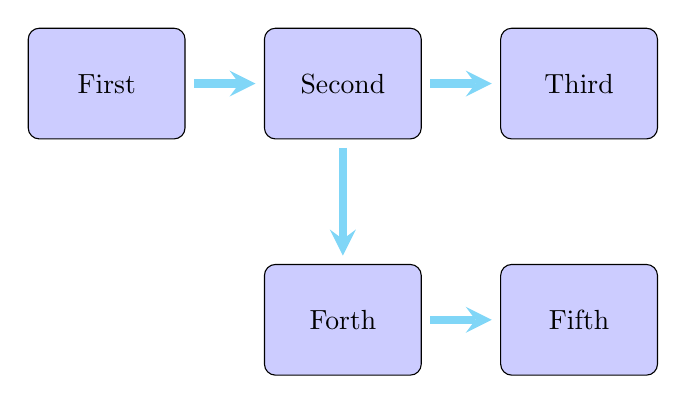
\begin{tikzpicture}[node distance=3cm,shorten >=3pt,shorten <=3pt]  
    
    \node[block]  (n1)  {First};  
    \node[block, right of=n1]  (n2) {Second};  
    \node[block, right of=n2] (n3) {Third};  
    \node[block, below of=n2] (n4) {Forth};  
    \node[block, below of=n3] (n5) {Fifth};  
    
    \begin{scope}[>=stealth,line width=3pt]
    \draw[->, cyan!50] (n1)  -- (n2);  
    \draw[->,cyan!50] (n2) -- (n3);  
    \draw[->,cyan!50] (n2) -- (n4);  
    \draw[->,cyan!50] (n4) -- (n5);  
    \end{scope}

  \end{tikzpicture}
\end{document}